\chapter{Goals and Constraints}
\label{chap:goals_constraints}

\section{Project Goals}
\label{sec:goals}
%What function(s) does the subsystem have to fulfill?

The principal goal of the \ac{U-SPACE} project is to try and bridge the gap between a student-driven engineering project and the concept of an unmanned \ac{SPA}. As very few examples of this type of design exist \cite{website:solr}, much is to be gained from this project. Due to the many constraints that have to been taken into account (see section \ref{sec:constraints}), the goal is necessarily modest. The goal of this project is thus designing, building and testing a small-scale \ac{SPA} for low altitude flight, including support for a scientific payload. The basic targets are listed below:

\begin{itemize}
\item Design of a small unmanned \ac{SPA} capable of forward propulsion, powered by solar cells and including a scientific payload
\item Construction of such an \ac{SPA} with minimal cost
\item Flight test of this \ac{SPA} at low altitude
\end{itemize}

\section{Project Constraints}
\label{sec:constraints}
%What technical requirements constrain the subsystem design? - e.g. mass, power, strength, stability etc.

The design, construction and test of a small unmanned \ac{SPA} is susceptible to many constraints, all of which have to be identified, examined and finally dealt with. These constraints take many forms, but may be divided into four categories: functionality, resources, environment and law.

\subsection{Functionality}

The \ac{U-SPACE} project, being a proof of concept, consists of designing, building and testing a small version of a \ac{SPA} with a limited scientific payload. Therefore reasonable limits have to be taken into account for some technical parameters. These parameters and their limits are listed below in table \ref{tab:functionality}.

\begin{table}[H]
\centering
\caption{Functional parameters and limits}
\label{tab:functionality}
\begin{tabular}{c c c}
\hline
\textbf{Parameter} & \textbf{Lower limit} & \textbf{Upper limit}\\ \hline
Total mass & / & 4.5 kg\\
Flight altitude & 2 m & 100 m\\
Electrical power & / & 8 W\\
Forward velocity & / & 1 m/s\\
Radius & 10 m & /\\
\hline
\end{tabular}
\end{table}

\subsection{Resources}

Since the \ac{U-SPACE} project is a student project supported by \ac{LTU} and \ac{IRF}, the available resources are limited. This imposes stringent constraints on all phases of the project. The main resources can be identified as the three elements of the project management triangle, shown in figure \ref{fig:project_triangle}.

\begin{figure}[htbp!]
\centering
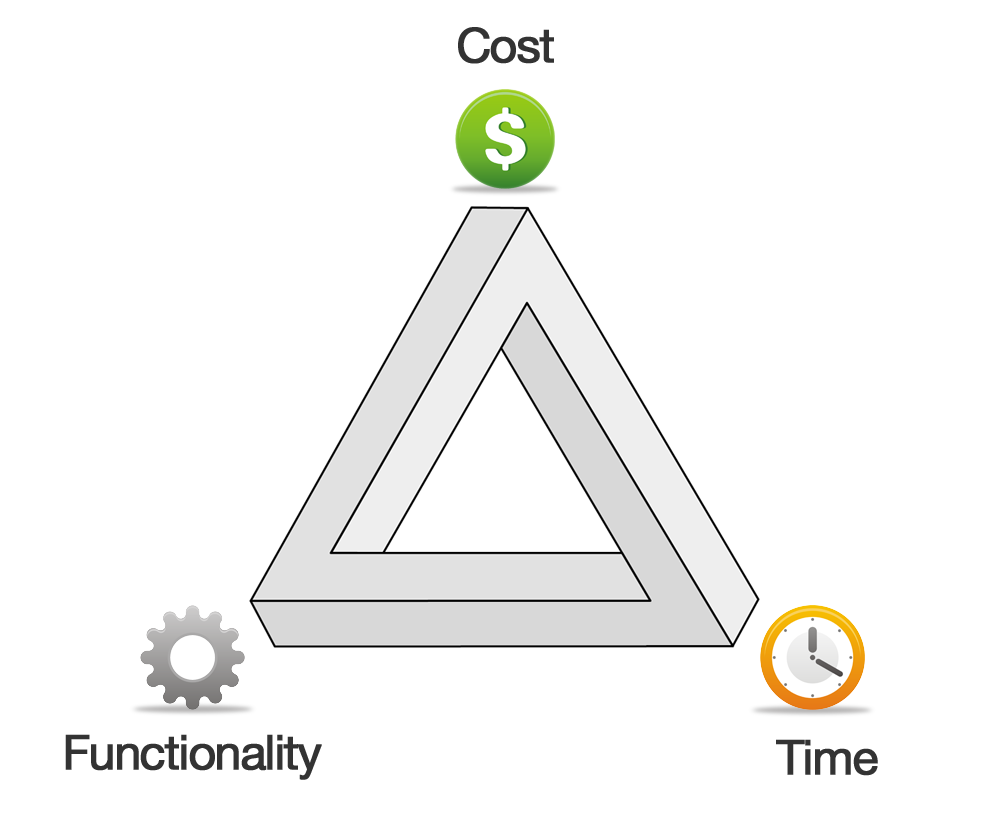
\includegraphics[scale=0.2]{figures/project_triangle.png}
\caption[Project management triangle]{Project management triangle \cite{website:claromentis}.}
\label{fig:project_triangle}
\end{figure}

\noindent
The cost of this student project is limited by its approved budget, a sum between 10,000 and 12,500 SEK, provided by \ac{LTU}. More funding can be applied for if required, but the budget nevertheless remains limited. This constraint implies a careful selection of components and the use of innovative engineering solutions throughout the entire project. 
\\
\\
The time available for this project is also constrained, being a student project that has to be realized in concurrence with other academic duties. The estimated time frame is therefore between 2 and 6 months for a first prototype capable of test flight.
\\
\\
The final resource is related to the previously mentioned functionality. With a limited number of team members that have limited expertise in the field of airships, the project has to be technically balanced, taking into account the capabilities of the members of the team.

\subsection{Environment}

The \ac{SPA} that will be developed during the \ac{U-SPACE} project finally has to be tested outdoors. Since the \ac{U-SPACE} project is being executed in the city of Kiruna during the spring, summer and early autumn, it is important to take the environmental conditions during this period of the year into account.  Some of the these conditions are listed below in table \ref{tab:environment}, using data for the month of May \cite{website:weatherspark} as a representation of the entire project period.

\begin{table}[H]
\centering
\caption{Environmental conditions}
\label{tab:environment}
\begin{tabular}{c c c c}
\hline
\textbf{Parameter} & \textbf{Lower boundary} & \textbf{Upper boundary} & \textbf{Remarks}\\ \hline
Temperature & -2 $^\circ$C & 11 $^\circ$C & Average values\\
Wind speed & 1 m/s & 6 m/s & Usually from the south west\\
Probability of precipitation & 61 \% & 61 \% & Average value\\
Hours of sunshine & 17:38 h & 22:45 h & Daily values\\
Cloud cover & 83 \% & 83 \% & Median value\\
Solar incidence angle & 46 $^\circ$ & 46 $^\circ$ & Refer to document USPACE-PDR-PWR-A1\\
\hline
\end{tabular}
\end{table}

\subsection{Law}

The final constraints that have to be taken into account are possible legal issues that may arise during the construction and testing of the \ac{SPA}. A first legal constraint is the compliance to the \ac{ITU} Radio Regulations \cite{book:freqalloc} when using wireless connections. Secondly, when flying the \ac{SPA}, the Swedish Transport Agency's regulations on \ac{UAS} \cite{regulations:uas2009} might have to be taken into account. As these application of these regulations depends on the final mass and size of the prototype airship, this constraint can only be investigated when a prototype is constructed.

\section{Expected Functionality}
%What are the expected performances of the subsystem, as related to the requirements above? (maybe including some margins)

Based on the project goals set forth in section \ref{sec:goals} and taking into account the constraints discussed in the previous section, a realistic prediction of the functionality of the final product of the \ac{U-SPACE} project can be made. The expected functionality of the small-scale \ac{SPA} are summarized in table \ref{tab:expected}.

\begin{table}[H]
\centering
\caption{Expected functionality}
\label{tab:expected}
\begin{tabular}{c c c c}
\hline
\textbf{Parameter} & \textbf{Value} & \textbf{Remarks}\\ \hline
Autonomy & 2 h & At peak power\\
Flight altitude & 2-20 m & /\\
Forward velocity & 0.5-1 m/s & /\\
Flight conditions & Daytime & Sunny and calm weather\\
\hline
\end{tabular}
\end{table}

\noindent
The other functional constraints presented in section \ref{sec:constraints} will be discussed in subsequent chapters. In the future, this functionality might be expanded with features like autonomous attitude control and altitude control during flight.

\section{Fault Tolerance Design and Safety Concept}

Since the goal of the \ac{U-SPACE} project is to design, build and test a prototype of a small-scale \ac{SPA} the focus of this project is not on a fault-tolerant design of the airship, but rather on a performant design that meets the project goals. Nevertheless some safety features are included in the design, construction and flight test of the airship. These features will be discussed in the chapters dedicated to the different subsystems and in chapter \ref{chap:ground_support}.

\section{Materials}

With the limited time and funding inherent to this student-driven project great care needs to taken with regards to the selection and processing of the materials. The materials need to be as performant as possible for their specific function while at the same time their cost should be as low as possible. In general all materials should also be as light as possible. The specific material requirements for each subsystem are discussed in the subsequent chapters.
\\
\\
With regards to the processing of the materials, low cost is again the main discriminator to select an appropriate technique. Therefore the simplest techniques are preferred during the construction of the airship, with as less mechanical work as possible. A certain amount of experience with such techniques is present in the team, allowing short construction times and limited delays.